
\section{RQ3}
\label{sec:RQ3}
\label{sec:generalization}

To examine how much OPD learning transfers to unseen
responses, we study three complementary aspects:
(1) \textbf{Validation Performance}, which tracks
how teacher KL and answer accuracy on held-out
questions evolve throughout training;
(2) \textbf{Transfer from Individual Updates}, which
measures the actual improvement produced by a single
training update on held-out responses, both in
magnitude and in the fraction of responses improved;
and (3) \textbf{Gradient Alignment Across Examples},
which examines how the directions of gradients from
training and validation examples, as well as different
training subsets, change during training.
We use the paired FULL trajectories at both scales,
with additional results and diagnostics reported in
Appendices~\ref{app:observations}
and~\ref{app:supplementary}.

\subsection{Validation Performance}
\label{sec:rq3_validation}
We first examine how performance on the excluded validation questions changes during training. At checkpoint $t$, the student generates a fresh response to each question. For a response $b$ containing $n_b$ positions, let $L_b(\theta)=n_b^{-1}\sum_i\ell_\theta(c_{bi})$. The validation loss averages these response losses, $K_V(\theta)=M^{-1}\sum_{b=1}^{M}L_b(\theta)$, where $M$ is the number of validation responses. Answer accuracy is the fraction of these responses with a correct final answer.

Validation KL decreases substantially at both scales, with the largest changes occurring early (Figure~\ref{fig:rq3_validation}a). Accuracy also improves early, followed by fluctuations over a narrower range (Figure~\ref{fig:rq3_validation}b). Table~\ref{tab:rq3_summary} summarizes the changes, and Table~\ref{tab:two_scale_validation} reports every observation. Continued agreement with the teacher therefore accompanies limited further improvement in sampled answer accuracy.

\begin{table}[t]
\centering
\caption{Validation performance and gradient alignment during
on-policy distillation. Validation metrics compare steps 10 and 106,
while single-update and gradient measurements compare steps 10 and 100.
Accuracy, relative KL improvement, and the fraction of improved
responses are reported as percentages.}
\label{tab:rq3_summary}
\footnotesize
\setlength{\tabcolsep}{2pt}
\begin{tabular}{lrr}
\toprule
Measurement & 1.7B & 4B \\
\midrule
Validation KL & $0.1742\!\to\!0.0784$ & $0.0976\!\to\!0.0445$\\
Validation accuracy & $7.03\!\to\!12.50$ & $25.78\!\to\!28.13$\\
Relative one-update gain & $7.20\!\to\!0.20$ & $6.53\!\to\!0.07$\\
Responses with lower KL & $100.00\!\to\!63.28$ & $98.44\!\to\!47.66$\\
Train--validation cosine & $0.913\!\to\!0.221$ & $0.922\!\to\!0.193$\\
Subset parameter cosine & $0.732\!\to\!0.083$ & $0.770\!\to\!0.060$\\
Subset hidden cosine & $0.898\!\to\!0.232$ & $0.889\!\to\!0.246$\\
Top-4 covariance overlap & $0.953\!\to\!0.890$ & $0.970\!\to\!0.947$\\
\bottomrule
\end{tabular}
\end{table}

\begin{figure*}[t]
\centering
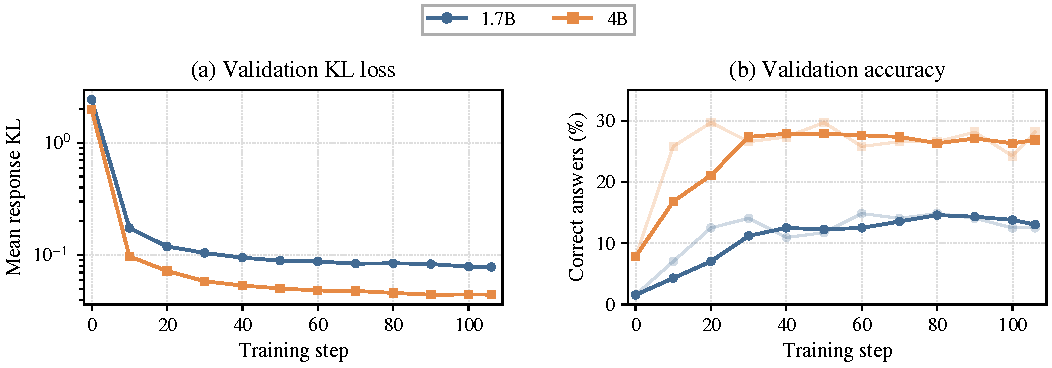
\includegraphics[width=\textwidth]{figures/rq3_validation.pdf}
\caption{Validation loss and answer accuracy over training.
At each checkpoint, the student generates new responses
to the same 128 held-out questions.
(a) Mean response KL on a logarithmic scale.
(b) Answer accuracy, with light lines showing individual
measurements and dark lines showing moving averages
over three observations.}
\label{fig:rq3_validation}
\end{figure*}

\subsection{Transfer from Individual Updates}
\label{sec:rq3_updates}

To measure the effect of individual training updates on
unseen responses, we evaluate validation KL loss before
and after the next actual AdamW update on a training batch.
At each checkpoint $t$, the student generates new responses
to held-out questions, which are kept fixed during the
before-and-after comparison.
Let $\theta_t^+=\theta_t+\Delta\theta_t$ denote the updated
parameters. We define the KL loss reduction for each
response and its average across validation responses as
\begin{equation}
 G_{b,t}=L_b(\theta_t)-L_b(\theta_t^+),\qquad
 G_{V,t}=\frac{1}{M}\sum_{b=1}^{M}G_{b,t}.
 \label{eq:rq3_gain}
\end{equation}
A positive $G_{b,t}$ indicates that the update reduces
the KL loss on response $b$.
We report the relative KL loss reduction
$G_{V,t}/K_V(\theta_t)$ and the fraction of responses
satisfying $G_{b,t}>10^{-6}$.
These metrics measure how much an update improves
validation responses and how many responses benefit.

The improvement from individual updates decreases
substantially over training
(Figure~\ref{fig:rq3_single_update}).
From checkpoint 10 to 100, the relative reduction
in validation KL loss drops from 7.20\% to 0.20\%
for 1.7B and from 6.53\% to 0.07\% for 4B
(Table~\ref{tab:rq3_summary}).
This decline persists after normalization by the
pre-update KL loss, indicating that each update
removes a smaller fraction of the remaining loss.
Some later updates even increase the mean validation
KL loss, despite its overall decrease throughout
training. Detailed results are reported in
Appendix~\ref{app:rq3_update_distribution}.

The fraction of responses benefiting from each update
also decreases. At checkpoint 10, nearly all validation
responses show lower KL loss after the update.
By checkpoint 100, this fraction falls to 63.28\%
for 1.7B and 47.66\% for 4B.
Notably, the 4B update still reduces the average
validation KL loss even though fewer than half of
the responses improve.
Thus, an average reduction in KL loss can mask
uneven improvements across unseen responses.
These measurements reflect changes in KL loss
on fixed responses rather than changes in
answer correctness.

\begin{figure*}[t]
\centering
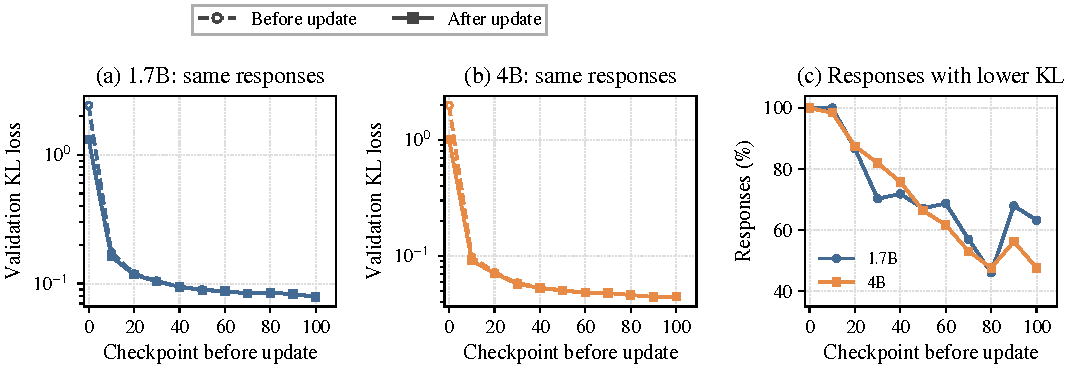
\includegraphics[width=\textwidth]{figures/rq3_single_update.pdf}
\caption{Effect of one actual training update on unseen responses. (a,b) Validation KL immediately before and after the update, evaluated on identical responses within each pair. Both axes for KL loss are logarithmic. The before/after curves approach each other as one-update improvements shrink. (c) Fraction of validation responses whose KL decreases by more than $10^{-6}$. The horizontal axis gives the checkpoint before the update; responses are freshly generated at each checkpoint and then fixed for its comparison.}
\label{fig:rq3_single_update}
\label{fig:two_scale_transfer}
\end{figure*}

\begin{figure*}[t]
\centering
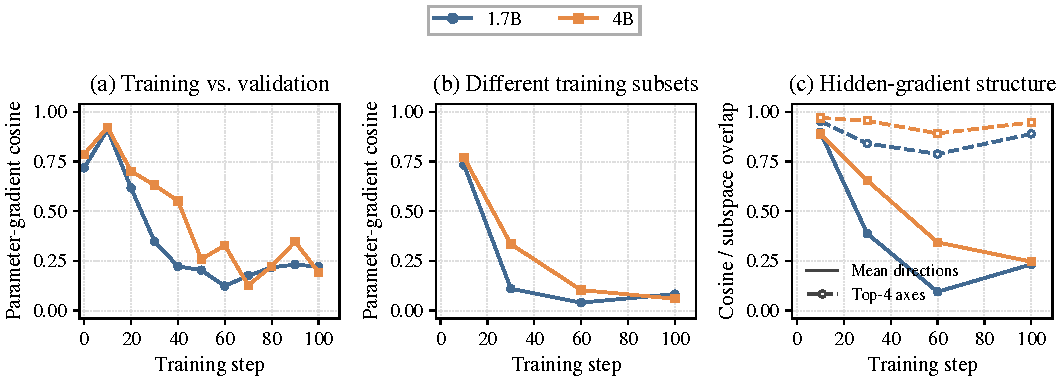
\includegraphics[width=\textwidth]{figures/rq3_gradient_agreement.pdf}
\caption{Gradient agreement during training. (a) Cosine between training and validation parameter gradients at the same checkpoint. (b) Mean parameter-gradient cosine across six pairs of four disjoint training subsets. (c) Mean cosine between subset-averaged hidden gradients and overlap of their top-4 centered covariance subspaces, using all hidden dimensions. Mean directions become less aligned while covariance axes remain similar. Lines connect the recorded observations.}
\label{fig:rq3_agreement}
\end{figure*}

\subsection{Gradient Alignment Across Examples}
\label{sec:rq3_agreement}

We next examine whether the declining benefit of
individual updates is accompanied by weaker gradient
alignment across examples.
Let $g_T$ be the training parameter gradient defined
in Section~\ref{sec:preliminaries and setup}, and
$g_V=\nabla_\theta K_V(\theta_t)$ the validation
parameter gradient at the same checkpoint.
We measure their alignment using cosine similarity:
\begin{equation}
 a_{TV,t}=\frac{g_T^\top g_V}{\|g_T\|_2\|g_V\|_2}.
 \label{eq:rq3_alignment}
\end{equation}
We also divide the training examples into four disjoint
subsets and compute their parameter gradients at the
same checkpoint. We report the average cosine similarity
across the six subset pairs to measure gradient alignment
among training examples.

Both measures of parameter-gradient alignment decrease
substantially during training
(Figure~\ref{fig:rq3_agreement}a,b;
Table~\ref{tab:rq3_summary}).
Late cross-subset cosine similarities are mostly small
and positive, with occasional negative values in 1.7B
(Table~\ref{tab:two_scale_batch}).
This decline accompanies the smaller transfer gains
observed in the preceding section.
However, weaker alignment does not necessarily imply
stronger conflict between examples: cosine similarity
can also decrease when mean gradients become small
relative to variation across examples.

To examine alignment at the representation level,
we also analyze gradients in the full hidden-state
space, as in RQ2.
For subset $b$, define the mean token gradient
$\mu_b=\mathbb E_b[g_h]$ and centered covariance
$\Sigma_b=\mathbb E_b[(g_h-\mu_b)(g_h-\mu_b)^\top]$.
We compare mean-gradient cosine similarities and
the overlap between leading covariance subspaces.
For top-$k$ eigenvector matrices $V_{a,k}$ and
$V_{b,k}$, subspace overlap is
$\|V_{a,k}^\top V_{b,k}\|_F^2/k$.

Mean hidden-gradient directions become less aligned,
while the leading covariance subspaces retain high
overlap at both scales
(Figure~\ref{fig:rq3_agreement}c).
The covariance subspaces describe the main directions
of gradient variation, whereas the mean gradients
indicate the average direction of the update signal
from each subset.
Thus, different subsets can share similar directions
of gradient variation even when their mean gradients
point in different directions.
Together, these results show that declining
single-update gains accompany weaker gradient
alignment across examples, despite the persistent
overlap in their covariance subspaces.
These observations do not establish a causal
relationship; identifying the cause of reduced
transfer requires controlling for gradient magnitude,
sampling variation, and the actual update direction.

\FloatBarrier
\begin{tcolorbox}[
 enhanced, breakable,
 colback=findingbg, colframe=findingblue,
 boxrule=0.7pt, arc=1.5mm,
 left=7pt, right=7pt, top=6pt, bottom=6pt,
 before skip=8pt, after skip=8pt
]
\textbf{\textcolor{findingblue}{Key Finding.}}
As OPD progresses, individual training updates
produce smaller reductions in KL loss on unseen
responses and improve fewer responses.
Meanwhile, gradients from different examples
become less aligned, although their dominant
directions of variation remain similar.
Validation KL loss continues to decrease,
while answer accuracy shows limited further
improvement in later training.
\end{tcolorbox}
